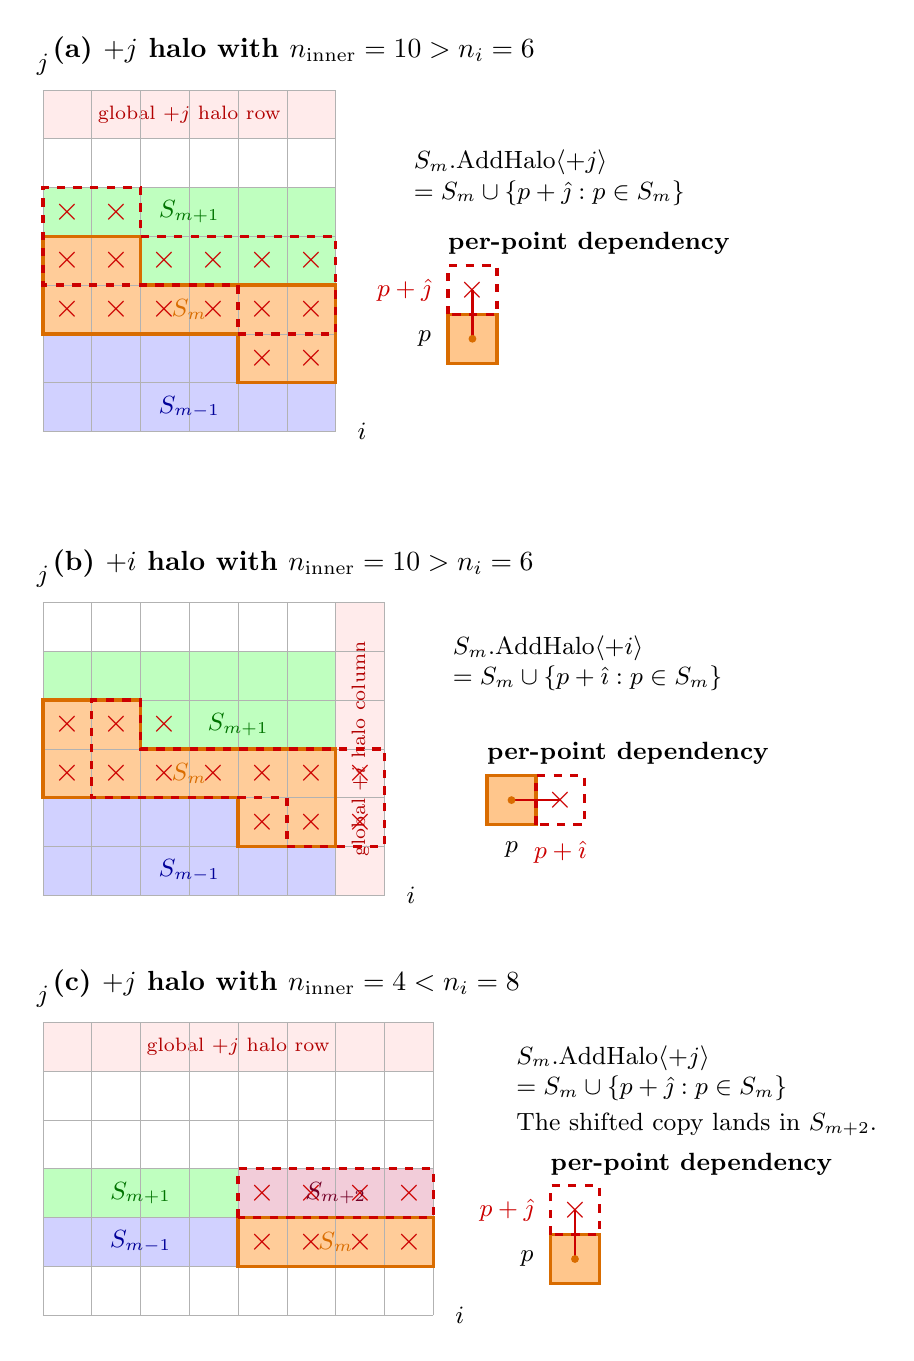
\begin{tikzpicture}[scale=0.62, every node/.style={font=\small}]
  % ============================================================
  % Visual convention:
  % blue    = previous inner range S_{m-1}
  % orange  = representative inner range S_m
  % green   = next inner range S_{m+1}
  % purple  = later inner range S_{m+2}
  % red x   = points visited by S_m.AddHalo<...>()
  % red dashed outline = shifted halo cells h(S_m)
  %
  % The drawn grid is the halo-extended logical domain.
  % ============================================================

  % ============================================================
  % Panel A: +j halo, ninner > ni
  % Original logical ni=6, nj=6. Extended grid has nj+1 rows.
  % ============================================================
  \begin{scope}[yshift=0cm]
    \def\ni{6}
    \def\njext{7}

    \node[font=\bfseries, anchor=west] at (0,7.8)
      {(a) $+j$ halo with $n_{\mathrm{inner}}=10>n_i=6$};

    % Halo-extended logical grid
    \draw[step=1, gray!45, very thin] (0,0) grid (\ni,\njext);

    % Original-domain inner ranges
    \fill[blue!18] (0,0) rectangle (6,1);
    \fill[blue!18] (0,1) rectangle (4,2);

    \fill[orange!40] (4,1) rectangle (6,2);
    \fill[orange!40] (0,2) rectangle (6,3);
    \fill[orange!40] (0,3) rectangle (2,4);

    \fill[green!25] (2,3) rectangle (6,4);
    \fill[green!25] (0,4) rectangle (6,5);

    % Mark globally added halo row
    \fill[red!8] (0,6) rectangle (6,7);
    \node[red!70!black, font=\scriptsize] at (3,6.5) {global $+j$ halo row};

    \draw[step=1, gray!60, very thin] (0,0) grid (\ni,\njext);

    % Boundary for S_m
    \draw[orange!85!black, very thick]
      (4,1) -- (6,1) -- (6,3) -- (2,3) -- (2,4) -- (0,4) -- (0,2) -- (4,2) -- cycle;

    % Shifted +j halo cells h(S_m)
    \draw[red!80!black, very thick, dashed]
      (4,2) -- (6,2) -- (6,4) -- (2,4) -- (2,5) -- (0,5) -- (0,3) -- (4,3) -- cycle;

    % S_m union shift_j(S_m)
    \foreach \i/\j in {
      4/1,5/1,
      0/2,1/2,2/2,3/2,4/2,5/2,
      0/3,1/3,2/3,3/3,4/3,5/3,
      0/4,1/4
    } {
      \node[red!80!black, font=\bfseries\large] at (\i+0.5,\j+0.5) {$\times$};
    }

    \node[blue!60!black] at (3,0.5) {$S_{m-1}$};
    \node[orange!85!black] at (3,2.5) {$S_m$};
    \node[green!45!black] at (3,4.5) {$S_{m+1}$};

    \node[anchor=west] at (6.25,0) {$i$};
    \node[anchor=south] at (0,7.1) {$j$};

    \node[align=left, anchor=west] at (7.4,5.2)
      {$S_m.\mathrm{AddHalo}\langle +j\rangle$\\
       $= S_m \cup \{p+\hat{\jmath}:p\in S_m\}$};

    % Per-point dependency inset
    \begin{scope}[xshift=8.3cm, yshift=1.4cm]
      \node[font=\small\bfseries, anchor=west] at (-0.2,2.45)
        {per-point dependency};

      \fill[orange!45] (0,0) rectangle (1,1);
      \draw[orange!85!black, very thick] (0,0) rectangle (1,1);
      \draw[red!80!black, very thick, dashed] (0,1) rectangle (1,2);

      \draw[red!80!black, thick] (0.5,0.5) -- (0.5,1.5);
      \fill[orange!85!black] (0.5,0.5) circle (0.08);
      \node[red!80!black, font=\bfseries\large] at (0.5,1.5) {$\times$};

      \node[anchor=east] at (-0.15,0.5) {$p$};
      \node[anchor=east, red!80!black] at (-0.15,1.5) {$p+\hat{\jmath}$};
    \end{scope}
  \end{scope}

  % ============================================================
  % Panel B: +i halo, ninner > ni
  % Original logical ni=6, nj=6. Extended grid has ni+1 columns.
  % ============================================================
  \begin{scope}[yshift=-9.5cm]
    \def\niext{7}
    \def\nj{6}

    \node[font=\bfseries, anchor=west] at (0,6.8)
      {(b) $+i$ halo with $n_{\mathrm{inner}}=10>n_i=6$};

    % Halo-extended logical grid
    \draw[step=1, gray!45, very thin] (0,0) grid (\niext,\nj);

    % Original-domain inner ranges
    \fill[blue!18] (0,0) rectangle (6,1);
    \fill[blue!18] (0,1) rectangle (4,2);

    \fill[orange!40] (4,1) rectangle (6,2);
    \fill[orange!40] (0,2) rectangle (6,3);
    \fill[orange!40] (0,3) rectangle (2,4);

    \fill[green!25] (2,3) rectangle (6,4);
    \fill[green!25] (0,4) rectangle (6,5);

    % Mark globally added halo column
    \fill[red!8] (6,0) rectangle (7,6);
    \node[red!70!black, rotate=90, font=\scriptsize] at (6.5,3)
      {global $+i$ halo column};

    \draw[step=1, gray!60, very thin] (0,0) grid (\niext,\nj);

    % Boundary for S_m
    \draw[orange!85!black, very thick]
      (4,1) -- (6,1) -- (6,3) -- (2,3) -- (2,4) -- (0,4) -- (0,2) -- (4,2) -- cycle;

    % Shifted +i halo cells h(S_m), geometrically shifted right.
    \draw[red!80!black, very thick, dashed]
      (5,1) -- (7,1) -- (7,3) -- (2,3) -- (2,4) -- (1,4) -- (1,2) -- (5,2) -- cycle;

    % S_m union shift_i(S_m)
    \foreach \i/\j in {
      4/1,5/1,6/1,
      0/2,1/2,2/2,3/2,4/2,5/2,6/2,
      0/3,1/3,2/3
    } {
      \node[red!80!black, font=\bfseries\large] at (\i+0.5,\j+0.5) {$\times$};
    }

    \node[blue!60!black] at (3,0.5) {$S_{m-1}$};
    \node[orange!85!black] at (3,2.5) {$S_m$};
    \node[green!45!black] at (4,3.5) {$S_{m+1}$};

    \node[anchor=west] at (7.25,0) {$i$};
    \node[anchor=south] at (0,6.1) {$j$};

    \node[align=left, anchor=west] at (8.2,4.75)
      {$S_m.\mathrm{AddHalo}\langle +i\rangle$\\
       $= S_m \cup \{p+\hat{\imath}:p\in S_m\}$};

    % Per-point dependency inset
    \begin{scope}[xshift=9.1cm, yshift=1.45cm]
      \node[font=\small\bfseries, anchor=west] at (-0.2,1.45)
        {per-point dependency};

      \fill[orange!45] (0,0) rectangle (1,1);
      \draw[orange!85!black, very thick] (0,0) rectangle (1,1);
      \draw[red!80!black, very thick, dashed] (1,0) rectangle (2,1);

      \draw[red!80!black, thick] (0.5,0.5) -- (1.5,0.5);
      \fill[orange!85!black] (0.5,0.5) circle (0.08);
      \node[red!80!black, font=\bfseries\large] at (1.5,0.5) {$\times$};

      \node[anchor=north] at (0.5,-0.15) {$p$};
      \node[anchor=north, red!80!black] at (1.5,-0.15) {$p+\hat{\imath}$};
    \end{scope}
  \end{scope}

  % ============================================================
  % Panel C: +j halo, ninner < ni
  % Original logical ni=8, nj=5. Extended grid has nj+1 rows.
  % ============================================================
  \begin{scope}[yshift=-18.1cm]
    \def\ni{8}
    \def\njext{6}

    \node[font=\bfseries, anchor=west] at (0,6.8)
      {(c) $+j$ halo with $n_{\mathrm{inner}}=4<n_i=8$};

    % Halo-extended logical grid
    \draw[step=1, gray!45, very thin] (0,0) grid (\ni,\njext);

    % Each range has length 4.
    \fill[blue!18]    (0,1) rectangle (4,2); % S_{m-1}
    \fill[orange!40]  (4,1) rectangle (8,2); % S_m
    \fill[green!25]   (0,2) rectangle (4,3); % S_{m+1}
    \fill[purple!20]  (4,2) rectangle (8,3); % S_{m+2}

    % Mark globally added halo row
    \fill[red!8] (0,5) rectangle (8,6);
    \node[red!70!black, font=\scriptsize] at (4,5.5) {global $+j$ halo row};

    \draw[step=1, gray!60, very thin] (0,0) grid (\ni,\njext);

    % Boundary for S_m
    \draw[orange!85!black, very thick]
      (4,1) rectangle (8,2);

    % Shifted +j halo cells h(S_m), coinciding with S_{m+2}
    \draw[red!80!black, very thick, dashed]
      (4,2) rectangle (8,3);

    % S_m union shift_j(S_m)
    \foreach \i/\j in {
      4/1,5/1,6/1,7/1,
      4/2,5/2,6/2,7/2
    } {
      \node[red!80!black, font=\bfseries\large] at (\i+0.5,\j+0.5) {$\times$};
    }

    \node[blue!60!black] at (2,1.5) {$S_{m-1}$};
    \node[orange!85!black] at (6,1.5) {$S_m$};
    \node[green!45!black] at (2,2.5) {$S_{m+1}$};
    \node[purple!60!black] at (6,2.5) {$S_{m+2}$};

    \node[anchor=west] at (8.25,0) {$i$};
    \node[anchor=south] at (0,6.1) {$j$};

    \node[align=left, anchor=west] at (9.5,4.6)
      {$S_m.\mathrm{AddHalo}\langle +j\rangle$\\
       $= S_m \cup \{p+\hat{\jmath}:p\in S_m\}$\\[2pt]
       {The shifted copy lands in $S_{m+2}$.}};

    % Per-point dependency inset, moved lower to avoid annotation overlap
    \begin{scope}[xshift=10.4cm, yshift=0.65cm]
      \node[font=\small\bfseries, anchor=west] at (-0.2,2.45)
        {per-point dependency};

      \fill[orange!45] (0,0) rectangle (1,1);
      \draw[orange!85!black, very thick] (0,0) rectangle (1,1);
      \draw[red!80!black, very thick, dashed] (0,1) rectangle (1,2);

      \draw[red!80!black, thick] (0.5,0.5) -- (0.5,1.5);
      \fill[orange!85!black] (0.5,0.5) circle (0.08);
      \node[red!80!black, font=\bfseries\large] at (0.5,1.5) {$\times$};

      \node[anchor=east] at (-0.15,0.5) {$p$};
      \node[anchor=east, red!80!black] at (-0.15,1.5) {$p+\hat{\jmath}$};
    \end{scope}
  \end{scope}
\end{tikzpicture}